% %
% stint-UserGuide.tex
% tutorial and other guide material for py-stint
%
%  Relies on REFMAN.CLS (LaTeX2e)
%
\documentclass[twoside,a4paper]{refart}
\usepackage{makeidx}
\usepackage{ifthen}
\usepackage{enumerate}
\usepackage{graphicx}
\usepackage{caption}
\usepackage{subcaption}
% ifthen wird vom Bild von N.Beebe gebraucht!

\def\bs{\char'134 } % backslash in \tt font.
\newcommand{\ie}{i.\,e.,}
\newcommand{\eg}{e.\,g..}
\DeclareRobustCommand\cs[1]{\texttt{\char`\\#1}}


\title{py-stint: PYthon Spatial/Temporal INtersection Toolset}
\author{IndEcol @ Norges teknisk-naturvitenskapelige universitet \\
Wiley Bogren \\
2014-09-05   \\
--- Version 1.1}

\date{}
\emergencystretch1em  %

\pagestyle{myfootings}
\markboth{User Guide to \textrm{py-stint}}%
         {User Guide to \textrm{py-stint}}

\makeindex 

\setcounter{tocdepth}{2}

\begin{document}

\maketitle

\begin{abstract}
        This document describes the capabilities and use of the 
        \texttt{py-stint} toolset for spatial and temporal 
        intersections.  The primary expected use for py-stint is 
        to produce datasets combining land-use and climate data 
        with MODIS albedo timeseries.
\end{abstract}


\tableofcontents

\newpage


%%%%%%%%%%%%%%%%%%%%%%%%%%%%%%%%%%%%%%%%%%%%%%%%%%%%%%%%%%%%%%%%%%%%


\section{Directory Structure}
\label{dirs}
The \texttt{py-stint} project relies on four essential directories.  
The user should have write access to \texttt{INPUT.txt} and \texttt{STINT/}. 
These directories can be located anywhere relative to each other, but the structure of each directory should be as follows:

\begin{description}
\item[\texttt{py-stint/}]
        \texttt{INPUT.txt}\\
        \texttt{run.py}\\
        \texttt{Tools/}\\
          \-\hspace{0.5cm} \texttt{*.py modules}\\
          \-\hspace{0.5cm} \texttt{Data/}\\
            \-\hspace{1.0cm} \texttt{MODIS\_tiles.shp}

\item[\texttt{MODIS\_ARCHIVE/}]
        \texttt{MCD43A3/}  --One directory per MODIS product\\
          \-\hspace{0.5cm} \texttt{h19v02/}  --One directory per MODIS tile\\
            \-\hspace{1.0cm} \texttt{*.hdf}

\item[\texttt{ERA\_ARCHIVE/}]
        \texttt{era\_climate\_t2m\_1of3.nc}\\
        \texttt{era\_climate\_t2m\_2of3.nc}\\
        \texttt{era\_climate\_t2m\_3of3.nc}\\
        \texttt{climate\_field2\_1of1.nc}
\item[\texttt{STINT/}]
        Holds output directories, which are made while running \texttt{py-stint}.
\end{description}

\section{Getting Data}
\label{data}
\index{data}

\subsection{Corine Landcover}\label{clc}
2006 Corine Land Cover seamless vector data is part of the European Commission programme to COoRdinate INformation on the Environment (Corine). 

EEA grants free access to all its data/applications provided that the user agrees:
\begin{itemize}
\item
to acknowledge the source as follows: Copyright EEA, Copenhagen, 2007

\item
to display a link to the EEA web site http://www.eea.europa.eu

\item
not to use the data/applications for commercial purposes unless the Agency has expressly granted the right to do so 
\end{itemize}
A spatialite database containing all landcover classes can be downloaded from the following link:

http://www.eea.europa.eu/data-and-maps/data/clc-2006-vector-data-version-3/


The spatialite database can be converted to shapefile and cropped to an Area of Interest via commandline:\\
\texttt{\$ ogr2ogr -f "ESRI Shapefile" <path/to/output> <path/to/clc06.sqlite> -dsco SPATIALITE=yes -clipsrc <xmin> <ymin> <xmax> <ymax>}


Where \texttt{<xmin> <ymin> <xmax> <ymax>} are the bounding x and y coordinates of the Area of Interest, in the LAEA-ETRS89 projection.

\subsection{ERA-Interim Climate}\label{era}
ERA Interim climate data can be downloaded from the following website. The server may require an user account before allowing the download.  

download:
http://apps.ecmwf.int/datasets/data/interim\_full\_daily/

terms of use:
http://apps.ecmwf.int/datasets/data/interim\_full\_daily/licence/


\attention
The ECMWF server sets a limit of about 2GB per file download.  Download data in netcdf format, in either 6-hour or 24-hour resolution, with a single field (attribute) per file. 

If the desired timespan will not fit on a single file, break it into as many downloads as necessary, with the start-date of each successive file one time-step later than the end-date of the previous file. e.g. if file1 ends 18:00 31. December 2011, then file2 should start 00:00 1. January 2012.

\subsection{MODIS Datasets}\label{modis}
MODIS products can be downloaded from two main sources, given below.  Future versions of \texttt{py-stint} will incorporate dataset retrieval tools and functions based on the \texttt{modis\_download.py} script from the \texttt{pyModis} project:
\texttt{http://pymodis.fem-environment.eu/}

For now the best plan is to either figure out \texttt{modis\_download.py} yourself (recommended, as it is excellent) or to (1) write a script in python or R to compile a list of files you want to download, then (2) use a command line utility like \texttt{axel} to retrieve all the files in the list.

After all files have been retrieved, ensure that the \texttt{MODIS\_Archive/} directory is organized in the \texttt{archive/product/tile/*.hdf} structure, as illustrated in Section \ref{dirs}. 

Core MODIS products such as albedo and surface temperature:\\
\texttt{http://e4ftl01.cr.usgs.gov/MOTA/}


Snow cover (National Snow and Ice Data Center):\\
\texttt{ftp://n5eil01u.ecs.nsidc.org/MOST/}

\newpage
\section{Workflow}\label{run}
Python programs given in the workflow guide should be called from the 
\texttt{py-stint/} directory.  These commands are presented in the format \\
\texttt{\$ python \ldots}


\subsection{Setup}

\begin{itemize}
    \item
        \texttt{\$ python Tools/MODIS\_aoi.py path/to/aoi.shp}
        \begin{itemize}
            \item
                Print a list of \texttt{MODIS} tiles to include in 
                \texttt{MODIS\_ARCHIVE/}
        \end{itemize}
    
    \item
        Create project directory
    \item
        Prepare \texttt{ERA} and \texttt{MODIS} archives 
        as per Section \ref{data}.  \\
        \texttt{MODIS\_ARCHIVE/} should be complete
        with regard to:
        \begin{itemize}
        \item
            products (MCD43A3 etc)
        \item
            dates within timeframe
        \item
            \texttt{MODIS} tiles which have been identifed within the \texttt{AOI}
        \end{itemize}
    \item
        Fill out \texttt{INPUT.ex} with actual project parameters, 
        then save as \texttt{py\_stint/INPUT.txt}
\end{itemize}


\subsection{Processing}
\label{stages}
After completing the setup, execute each of the 7 processing stages 
consecutively via the command line.

\subsubsection{\textbf{Stage 1:} \texttt{\$ python run.py 1}}
The stage begins by parsing project parameters from \texttt{INPUT.txt}, 
as well as loading the projection and extent from the area of interest 
(\texttt{AOI}). Technically, these are loaded at the start of every stage, 
but this is where you'll be alerted to any errors in the input parameters.

The stage then checks for corrupt or missing files within the 
\texttt{MODIS\_archive} given the region, timeframe and datasets 
specified in the input parameters.

Finally, the time variable is loaded from each NetCDF file in the 
\texttt{ERA} archive.  An error is raised if there are any gaps 
or overlaps in timesteps.


  \begin{description}
    \item [Requires]
          \texttt{INPUT.txt} \\
          \texttt{AOI}/landcover shapefile \\
          \texttt{MODIS\_archive} \\
          \texttt{ERA\_archive} \\
          \texttt{MODIS\_tiles.shp}
      
  
  
    \item [Produces]
      Prints a report on any issues found in the 
      \texttt{MODIS} or \texttt{ERA} archives.
      
      Creates subdirectories within the \texttt{STINT/} directory, 
      if they are not already present.
      

    \item [Explore]
      This stage produces no new data to explore.
  \end{description}
  
\subsubsection{\textbf{Stage 2:} \texttt{\$ python run.py 2}}
This stage aggregates each \texttt{MODIS} and \texttt{ERA} dataset into
a single HDF5 array file, with dimensions [time, y, x].

The [time] dimension is shared by \texttt{MODIS} and \texttt{ERA} arrays, each timestep covering one 16-day \texttt{MODIS} observation period.

The spatial dimensions [y,x] are defined by the dataset's 
native projection (\texttt{MODIS sinusoidal} or \texttt{WGS84} geographic coordinates).
        
HDF5 arrays are cropped to the project timeframe and the minimum 
rectangle necessary to completely contain the \texttt{AOI}.


\texttt{MODIS} datasets: tiles are merged, subsets determined, and days aggregated.

\texttt{ERA} datasets: subsets determined, 6- or 24-hour records averaged to match 16-day \texttt{MODIS} intervals.

  \begin{description}
    \item [Requires]
          \texttt{INPUT.txt} \\
          \texttt{AOI}/landcover shapefile \\
          \texttt{MODIS\_archive} \\
          \texttt{ERA\_archive} \\
          \texttt{MODIS\_tiles.shp}
  
  
    \item [Produces]
      \texttt{ERA} and \texttt{MODIS} HDF5 array files, native projections:\\
      \texttt{STINT/Processing/HDF/<dataset>.hdf5}
      

    \item [Explore]
      The HDF5 array file is probably the richest, most exciting format 
      generated in \texttt{py-stint} processing. Data for a given region 
      and timeframe is stored in a single, compact and efficient format. 
      It has excellent potential for visualization of spatial and temporal 
      trends within albedo and climate datasets. 
      
      The first tool for exploring HDF5 data will be a python program for
       converting individual timesteps to geoTIFF files, which can be 
       viewed in a desktop GIS browser.
      
      
      * Python: h5py and numpy
      
      * R: rhdf5, h5r, or ncdf4 
      
      * matlab: h5disp and h5read
  \end{description}


\subsubsection{\textbf{Stage 3:} \texttt{\$ python run.py 3}}
Produce \texttt{ERA} and \texttt{MODIS} shapefiles from HDF5 subset arrays.
 
The shapefiles consist of a polygon grid, each raster cell represented by
rectangle with attribute fields for cell id, cell center coordinates, and grid coordinates which allow cell values to be retrieved from the HDF5 array file.  For example  \texttt{y\_ind} = 0, \texttt{x\_ind} = 0 is the top left cell in the grid.
 
The spatial reference system of the shapefile geometries as well as the cell center coordinates is the same as the HDF5 from which the grid was derived, \texttt{MODIS} sinusoidal or \texttt{ERA WGS84}.

  \begin{description}
    \item [Requires]
          \texttt{STINT/Processing/HDF/<project>\_<dataset>.hdf5}
  
  
    \item [Produces]
      \texttt{ERA} and \texttt{MODIS} shapefiles, native projections:\\
      \texttt{STINT/Processing/SHP/<project>\_era.shp} \\
      \texttt{STINT/Processing/SHP/<project>\_modis.shp} 
      

    \item [Explore]
      The products of this stage are standard ESRI shapefiles that can be explored in any GIS browser.  Attribute fields and projection of each file are summarized below:
      
\begin{tabular}{ll}
       \multicolumn{2}{c}{\texttt{modis.shp}} \\
Spatial reference system        & \texttt{MODIS} sinusoidal projection \\
\texttt{id}                     & \texttt{MODIS} cell id \\  
\texttt{x\_ctr},\texttt{y\_ctr} &  (x, y) sinusoidal coordinates, cell center\\
\texttt{x\_ind},\texttt{y\_ind} & grid coordinate HDF5 array file\\
\end{tabular}
      
\begin{tabular}{ll}
       \multicolumn{2}{c}{ \texttt{era.shp}} \\
Spatial reference system        & \texttt{WGS84} geographic coordinates \\
\texttt{id}                     & \texttt{ERA} cell id\\
\texttt{x\_ctr},\texttt{y\_ctr} & (lon, lat) coordinates, cell center \\ 
\texttt{x\_ind},\texttt{y\_ind} & grid coordinate HDF5 array file\\
\end{tabular}

  \end{description}


\subsubsection{\textbf{Stage 4:} \texttt{\$ python run.py 4}}
Transform \texttt{ERA} \& \texttt{MODIS} shapefiles to \texttt{AOI}/landcover spatial reference system.
        
Construct r-tree spatial index (\texttt{*.idx}) for each to speed up spatial queries such as the intersection in Stage 5.

Cell center coordinates in the attribute fields \texttt{y\_ctr} and \texttt{y\_ctr} remain in the dataset's original spatial reference system.

  \begin{description}
    \item [Requires]
      \texttt{STINT/Processing/SHP/<project>\_era.shp}\\
      \texttt{STINT/Processing/SHP/<project>\_modis.shp}
  
    \item [Produces]
      \texttt{ERA} and \texttt{MODIS} shapefiles with index, 
      \texttt{AOI} projections:\\ 
      \texttt{STINT/Processing/SHP/<project>\_era\_reprj.shp}\\
      \texttt{STINT/Processing/SHP/<project>\_era\_reprj.idx}\\
      \texttt{STINT/Processing/SHP/<project>\_modis\_reprj.shp}\\
      \texttt{STINT/Processing/SHP/<project>\_modis\_reprj.idx}      
      

    \item [Explore]
      The products of this stage are standard ESRI shapefiles that can be explored in any GIS browser.  Attribute fields and projection of each file are summarized below:
      
\begin{tabular}{ll}
       \multicolumn{2}{c}{\texttt{modis\_reprj.shp}} \\
Spatial reference system        & Native \texttt{AOI} projection \\
\texttt{id}                     & \texttt{MODIS} cell id \\  
\texttt{x\_ctr}, \texttt{y\_ctr} & (x, y) sinusoidal coordinates, cell center \\
\texttt{x\_ind}, \texttt{y\_ind} & grid coordinate HDF5 array file\\
\end{tabular}
      
\begin{tabular}{ll}
       \multicolumn{2}{c}{ \texttt{era\_reprj.shp}} \\
Spatial reference system        & Native \texttt{AOI} projection \\
\texttt{id}                     & \texttt{ERA} cell id\\
\texttt{ctr\_x}, \texttt{ctr\_y} & (lon, lat) coordinates, cell center \\ 
\texttt{x\_ind}, \texttt{y\_ind} & grid coordinate HDF5 array file\\
\end{tabular}

  \end{description}


\subsubsection{\textbf{Stage 5:} \texttt{\$ python run.py 5}}
Intersect \texttt{AOI}/landcover shapefile with \texttt{era\_reprj.shp} to produce landcover/climate shapefile, \texttt{lcc.shp}.  Each feature in the intersection product is wholly within a single ERA climate cell and a single landcover type.
          
Attribute fields specified by \texttt{lc\_} in \texttt{INPUT.txt} are preserved from \texttt{AOI}/landcover shapefile.
          
Takes advantage of \texttt{era\_reprj.idx} to speed up intersection.

  \begin{description}
    \item [Requires]
      \texttt{AOI}/landcover shapefile\\
      \texttt{STINT/Processing/SHP/<project>\_era\_reprj.shp}\\
      \texttt{STINT/Processing/SHP/<project>\_era\_reprj.idx}  
  
  
    \item [Produces]
      land cover/climate shapefile with index, 
      \texttt{AOI} projection:\\
      \texttt{STINT/Processing/SHP/<project>\_lcc.shp}\\
      \texttt{STINT/Processing/SHP/<project>\_lcc.idx}

    \item [Explore]
      \texttt{lcc.shp} is a standard ESRI shapefile that can be explored in any GIS browser.  Attribute fields and projection are summarized below:
      
\begin{tabular}{ll}
       \multicolumn{2}{c}{\texttt{lcc.shp}} \\
Spatial reference system        & Native \texttt{AOI} projection \\
\texttt{id}                     & lcc cell id \\  
\texttt{era\_id}                & \texttt{ERA} cell id \\  
\texttt{era\_ctr\_x}, \texttt{era\_ctr\_y} & (lon, lat) coordinates, \texttt{ERA} cell center \\
\texttt{era\_x\_ind}, \texttt{era\_y\_ind} & grid coordinate of matching record \\
                                          & from \texttt{ERA} HDF5 array file\\
\\
\texttt{lc\_id}                & \texttt{AOI}/landcover feature id \\
\texttt{lc\_*}                & Any attribute fields, such as land type, \\
                             & selected for preservation \\
                             & from \texttt{AOI}/landcover shapefile \\

\end{tabular}
  \end{description}


\subsubsection{\textbf{Stage 6:} \texttt{\$ python run.py 6}}
        Intersect \texttt{lcc.shp} with \texttt{modis\_reprj.shp} to produce landcover/climate/modis shapefile, \texttt{lcm.shp}. 
        
        Each feature in the intersection product is wholly within a single \texttt{MODIS} cell, single \texttt{ERA} climate cell, and a single landcover type. This combination of attribute fields is illustrated in Figure \ref{fig:lcm}.
          
Attribute fields from \texttt{lcc.shp} are preserved, as well as additionl fields identifying which MODIS cell each feature belongs to.  Additionally, an Area field describes the size in square meters of each feature in the aoi projection.
          
Takes advantage of \texttt{modis\_reprj.idx} to speed up intersection.
        
        \texttt{lcm.shp} is effectively the central product of this workflow,
          breaking each landcover feature into polygons wholly within and
          linked to individual MODIS and ERA cells

  \begin{description}
    \item [Requires]
      \texttt{STINT/Processing/SHP/<project>\_modis\_reprj.shp} \\
      \texttt{STINT/Processing/SHP/<project>\_modis\_reprj.idx} \\
      \texttt{STINT/Processing/SHP/<project>\_lcc.shp}
  
  
    \item [Produces]
      landcover/climate/modis shapefile with index, 
      \texttt{AOI} projection:\\
      \texttt{STINT/Processing/SHP/<project>\_lcm.shp}\\
      \texttt{STINT/Processing/SHP/<project>\_lcm.idx}
      

    \item [Explore]
      \texttt{lcm.shp} is a standard ESRI shapefile that can be explored in any GIS browser.  Attribute fields and projection are summarized below:
      
\begin{tabular}{ll}
       \multicolumn{2}{c}{\texttt{lcm.shp}} \\
Spatial reference system        & Native \texttt{AOI} projection \\
\texttt{id}                     & lcc cell id \\
\texttt{area}                   & area of feature in \texttt{AOI} projection, m\textsuperscript{2}\\  
\\
\texttt{era\_id}                & \texttt{ERA} cell id \\  
\texttt{era\_ctr\_x}, \texttt{era\_ctr\_y} & (lon, lat) coordinates, \texttt{ERA} cell center \\
\texttt{era\_x\_ind}, \texttt{era\_y\_ind} & grid coordinate of matching record \\
                                          & from \texttt{ERA} HDF5 array file\\
\\
\texttt{mod\_id}                & \texttt{MODIS} cell id \\  
\texttt{mod\_ctr\_x}, \texttt{mod\_ctr\_y} & (x, y) coordinates, \texttt{MODIS} cell center \\
\texttt{mod\_x\_ind}, \texttt{mod\_y\_ind} & grid coordinate of matching record \\
                                          & from \texttt{MODIS} HDF5 array file\\
\\
\texttt{lc\_id}                & \texttt{AOI}/landcover feature id \\
\texttt{lc\_*}                & Any attribute fields, such as land type, \\
                             & selected for preservation \\
                             & from \texttt{AOI}/landcover shapefile \\
\end{tabular}

\begin{figure}
\label{fig:lcm}
        \centering
        \begin{subfigure}[b]{0.3\textwidth}
                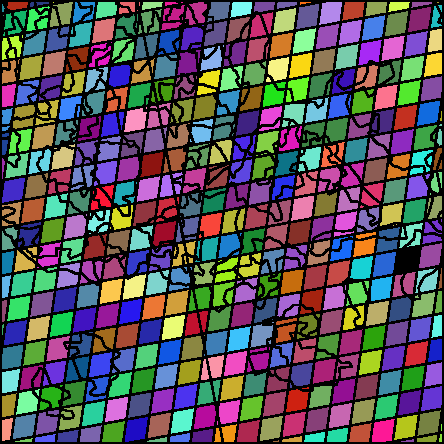
\includegraphics[width=\textwidth]{thumbs/lcm_modis}
                \caption{\texttt{MODIS} id}
                \label{fig:lcm-mod}
        \end{subfigure}
        ~ 
        \begin{subfigure}[b]{0.3\textwidth}
                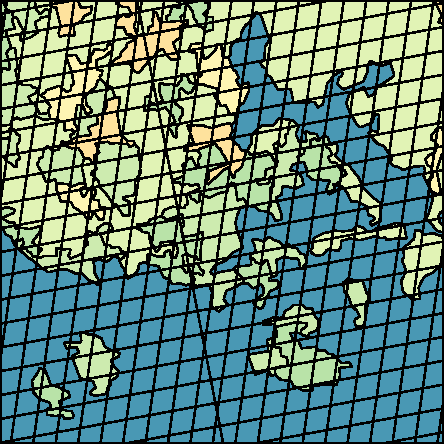
\includegraphics[width=\textwidth]{thumbs/lcm_landcover}
                \caption{Landcover}
                \label{fig:lcm-landcover}
        \end{subfigure}
        ~ 
        \begin{subfigure}[b]{0.3\textwidth}
        
                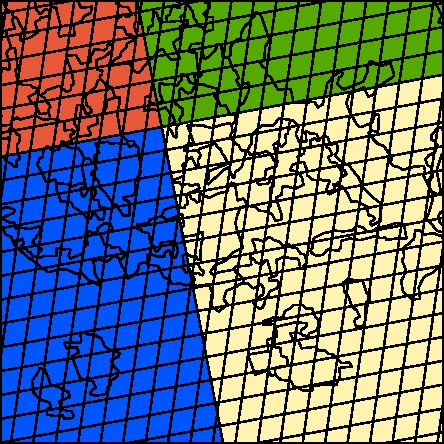
\includegraphics[width=\textwidth]{thumbs/lcm_era}
                \caption{\texttt{ERA} id}
                \label{fig:lcm-era}
        \end{subfigure}
       
        \caption{\texttt{lcm.shp}, shaded by different attribute fields}\label{fig:lcm}
\end{figure}
  \end{description}



\subsubsection{\textbf{Stage 7:} \texttt{\$ python run.py 7}}
  This stage exports a CSV spreadsheet file for each 
  \texttt{MODIS} and \texttt{ERA} dataset, 
  corresponding to the HDF5 array files, 
  as well as an additional landcover CSV which gives the area of each feature in 
  \texttt{lcm.shp} and links the feature to the corresponding 
  \texttt{MODIS} and \texttt{ERA} rows 
  (each row representing one raster cell across time)
  
  The CSV system is basically a two dimensional representation of the 
  HDF5 array files combined with \texttt{lcm.shp}.  Each row in \texttt{lc.csv} 
  represents a single feature in \texttt{lcm.shp}, with landcover attributes 
  as well as the \texttt{MODIS\_id} and \texttt{ERA\_id} linked to the feature.

  Each \texttt{MODIS} and \texttt{ERA} cell identified in \texttt{lcm.shp}
  is represented as a row within 
  each of the respective dataset CSV files, with columns corresponding to \texttt{MODIS} 
  intervals within the timeframe specified.
  
%  For projects with more than 20k landcover features, the exported CSVs are broken up into regions, each made up of 50 \texttt{MODIS} cells.  In this case, the filename is structured as \texttt{<project>\_<dataset>\_<region\_number>.csv}
  
  \begin{description}
    \item [Requires]
      \texttt{AOI}/landcover shapefile \\
      \texttt{STINT/Processing/HDF/<project>\_<dataset>.hdf5} \\
      \texttt{STINT/Processing/SHP/<project>\_lcm.shp}
  
  
    \item [Produces]
      \texttt{STINT/Output/CSV/<project>\_lc.csv} \\
      \texttt{STINT/Output/CSV/<project>\_<dataset>.csv}
      
    \item [Explore]
\texttt{lc.csv}: each row is a landcover feature with \texttt{MODIS} and \texttt{ERA} links
        
\texttt{MODIS} and \texttt{ERA} dataset CSVs: each row is a full timeseries for an
          individual cell identified within \texttt{lcm.shp}.
          
  \end{description}


%\clearpage
\subsection{Troubleshooting}
While I tried hard to write code that catches problems and prints clear messages describing the nature of the error, there may be situations where unclear errors slip through.  If such errors emerge while running \texttt{py-stint}, they will probably come in one of the following flavors:
\begin{enumerate}
  \item
    Input: a problem with the format or structure of input parameters, 
    project directories, or files linked to the project.  
    
    Going through the INPUT.txt file and the directory structure 
    can help resolve this kind of error.
  \item
    File Access: a problem opening or loading the contents of a file, 
    such as a shapefile or hdf.  
    
    This can arise through an input error, a problem with the 
    installation of the module being used to access the data,
    or a problem with the library that module depends on.
  \item
    Data Operations: a problem manipulating or transforming data, 
    such as managing data types, transforming spatial coordinates or 
    geometries between projections, or sorting multiple 
    \texttt{MODIS} arrays into a single subset array.
    
    This could be due to a module/library installation problem, or 
    because of a previous failed operation. Errors do not always end the process 
    at the point when they occur. It could be that a file access or 
    transformation step failed earlier in the processing, but the 
    resulting incorrect or None type object did not immediately provoke an 
    error or Exception.
    
\end{enumerate}

Each stage described in Section \ref{stages} includes a list of input files in order to help in tracking down any errors that do arise.
% Could add an item listing modules called from \texttt{py-stint/Tools/}?
% Could add an item listing potential errors? eg:
%% loading srs
%% transforming coordinates between srs
%% reading gdal formats (MODIS hdf)



% Commands shifting sections to Appendices, and labelling Appendix as such
\clearpage
\section*{Appendix}
\addcontentsline{toc}{section}{Appendix}
\appendix
\section{Requirements \& Installation}
\label{setup}
\index{setup}

Python 2.7 is required for \texttt{py-stint}.

On an Ubuntu system, the following commands are sufficient to set up the libraries and python modules listed in Sections \ref{libraries} and \ref{python-modules}.

\texttt{\$ sudo apt-get install ipython python-numpy python-pip python-scipy python-matplotlib python-h5py python-software-properties}

\texttt{\$ sudo add-apt-repository ppa:ubuntugis/ubuntugis-unstable}

\texttt{\$ sudo apt-get install libspatialindex-dev python-gdal gdal-bin}

\texttt{\$ sudo pip-install rtree pyproj}


\subsection{Library Dependencies}\label{libraries}
The following software libraries must be compiled before many 
of the python modules can be installed.  
When possible, try to compile them in the order listed, as some 
(such as gdal) have capabilities which depend on the previous 
libraries already being present.
\begin{description}

\item[GEOS]
        Required for geometric intersections.\\
        http://trac.osgeo.org/geos/

\item[libspatialindex]
        Required for rtree spatial indexing module for python.\\
        http://libspatialindex.github.io/

\item[netCDF4]
        Required for ERA climate data and gdal support for MODIS hdf.\\
        https://www.unidata.ucar.edu/software/netcdf/
        
\item[hdf5]
       Required for h5py and the format used 
       to aggregate MODIS and ERA subset arrays.\\
       http://www.hdfgroup.org/HDF5/
       
\item[GDAL]
        Required for geospatial data I/O.\\
        http://www.gdal.org/

\item[proj.4]
       required for reprojecting shapefile and raster datasets.\\
       http://trac.osgeo.org/proj/

\end{description}


\subsection{Python Dependencies}\label{python-modules}
Basic modules are included in most installations of python.  Scientific and Geospatial modules can be installed via package management, pip, or easyinstall. Geospatial modules in particular may require the libraries listed in Section \ref{libraries} to be available.
\begin{description}
\item[Basic Modules]
        os, sys, math, glob, multiprocessing, datetime, cPickle, csv

\item[Scientific Modules]
        numpy, scipy, netCDF4, h5py

\item[Geospatial Modules]
        gdal+ogr+osr, rtree
     
\end{description}


\end{document}
